\section{Planning phase}
Planning the new Autograder took many iterations of design and layout. The programming phase is simplified if most parts of the user interface has been planned ahead. All actions, tasks and functions of the site must be mapped out. New functionality must also be incorporated into the new design. The next section will show how the new layout has been planned and designed.


\subsection{User stories}
The more traditional way of designing a website is to start with wireframes. Wireframes are basic sketches or mockups of the design. The most basic forms does not include colors or advanced shapes. Simple boxes and rectangles are used to get a feel for how the page will look and function. The process starts with a revisit of the old Autograder front-end. All functions and tasks of all users must be mapped out. This includes functions such as approval of labs, signing in, making groups etc. More basic functions like getting students from the server, listing them and so on is also written down. The tasks are mapped using a technique called \emph{User Stories}. User stories are verbal guides to map all functionality. Stories come in the form \emph{"As a <role>, I want to <goal> so that <benefit>"}. Here are some of the user stories that Autograder uses;

\begin{itemize*}
\item As a student I want to create new group, so that other students can join for group assignment.
\item As an admin I want to list all current students so that I can manage permissions (admin,teacher,student).
\item As a teacher I want to archive / delete course, so that I can see only relevant and active courses.
\end{itemize*}

(Note: A table of user stories can be found in Appendix \worry{Appendix ref for full list of user stories}).

User stories help plan the whole system. The order of which functions are implemented can be managed from the start. In Autograder's case, functions like listing labs for the teacher will be a high priority user story. Functions like changing the group names can wait until a later point in development. Spreadsheets can be a good way of writing down all the user stires. Each role of the page, i.e students, teachers and admins can be placed in different columns. User stories for each column is then written in rows. For the new Autograder front-end, Trello was used. Trello's card design allows for easy grouping of cards, as well as an interface for drag and drop. This makes the job of managing the user stories much more simple, and it can also be used throughout the development as a TODO list.

\begin{figure}[h!]
    \centering
    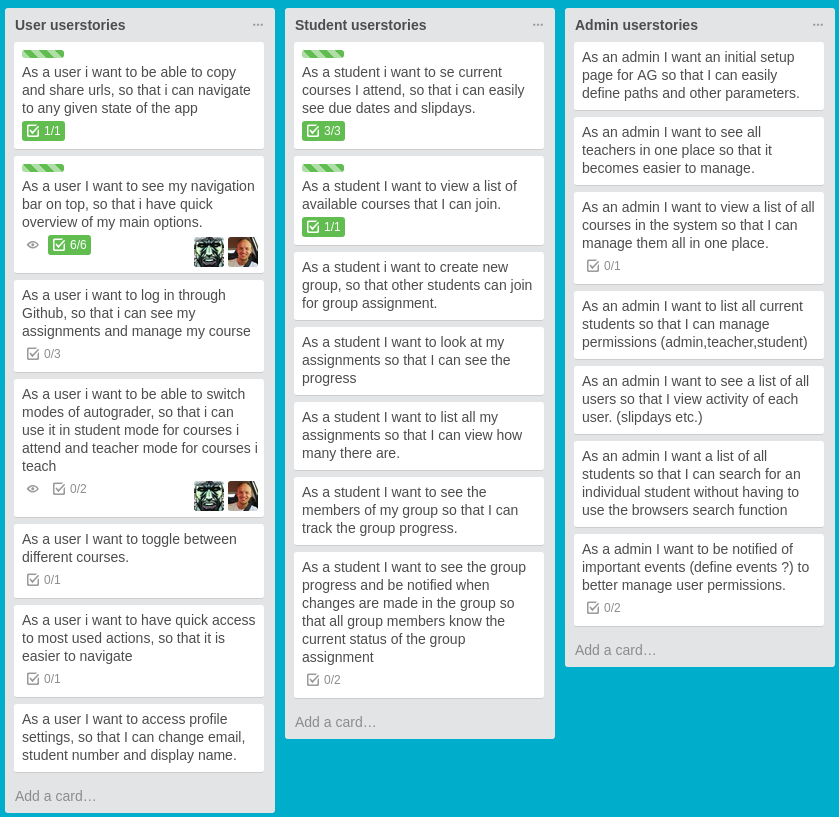
\includegraphics[width=0.8\textwidth]{./graphs/trello.png}
    \caption{Autograder's Trello page. Comprised of user stories, it was used as a TODO-list in the development process. Note: this is meant as an illustrative figure.}
    \label{fig:View of the trello page we used in the development process}
\end{figure}

\subsection{Wireframes}
The user stories are written down as cards. The user stories are then transformed into Wireframes are drawn as simple layouts with pen and paper. The client is present in the process to make sure the client and developers are on the same page. In our case, we talked to Professor Hein Meling at UiS, which acted as the client for the new Autograder. Pages such as the results view \worry{ref til figur/wireframe} went though many iterations before landing on the final layout. Not having to spend time on programming the site and changing the code, one can easily visualize the whole user interface before programming.

The wireframes are not to be confused with the design process. The wireframes are guides for user experience, not design. Having used the old Autograder system, we could use this previous experience to remake some of the layout. As said in the introduction \worry{ref til introduction}, limitations in the grading process was the main concern. Presenting the wireframes to the client will also make it easier to make rapid changes to the design, using a low-fidelity approach, with sketches and mock-ups. When the initial phase is done, more sophisticated drawings or wireframes are being created. These more detailed drawings with description of areas of the interface, describe what certain elements of the user interface does. Serving as a blueprint for further development. The next step in the process is to reflect the wireframes in code.

\subsection{The design}


\todo{}
